\chapter{OBDH}\label{ch:obdh}

The aim of this assignment is to experiment with
a reduced version of an On-Board Data Handling (OBDH) system
implemented on the UPMSat-2 microsatellite.
The OBDH is typically implemented by software,
which is also known as the On-Board Software (OBSW) of the satellite.
In this assignment,
the OBSW reads the MCU temperature using a temperature sensor
that is embedded in the MCU and connected to one of its ADCs.

\section{Software architecture}

The software architecture of the OBSW is depicted in \ref{fig:obdh}.
The software components are:

\begin{figure}[h]
	\centering{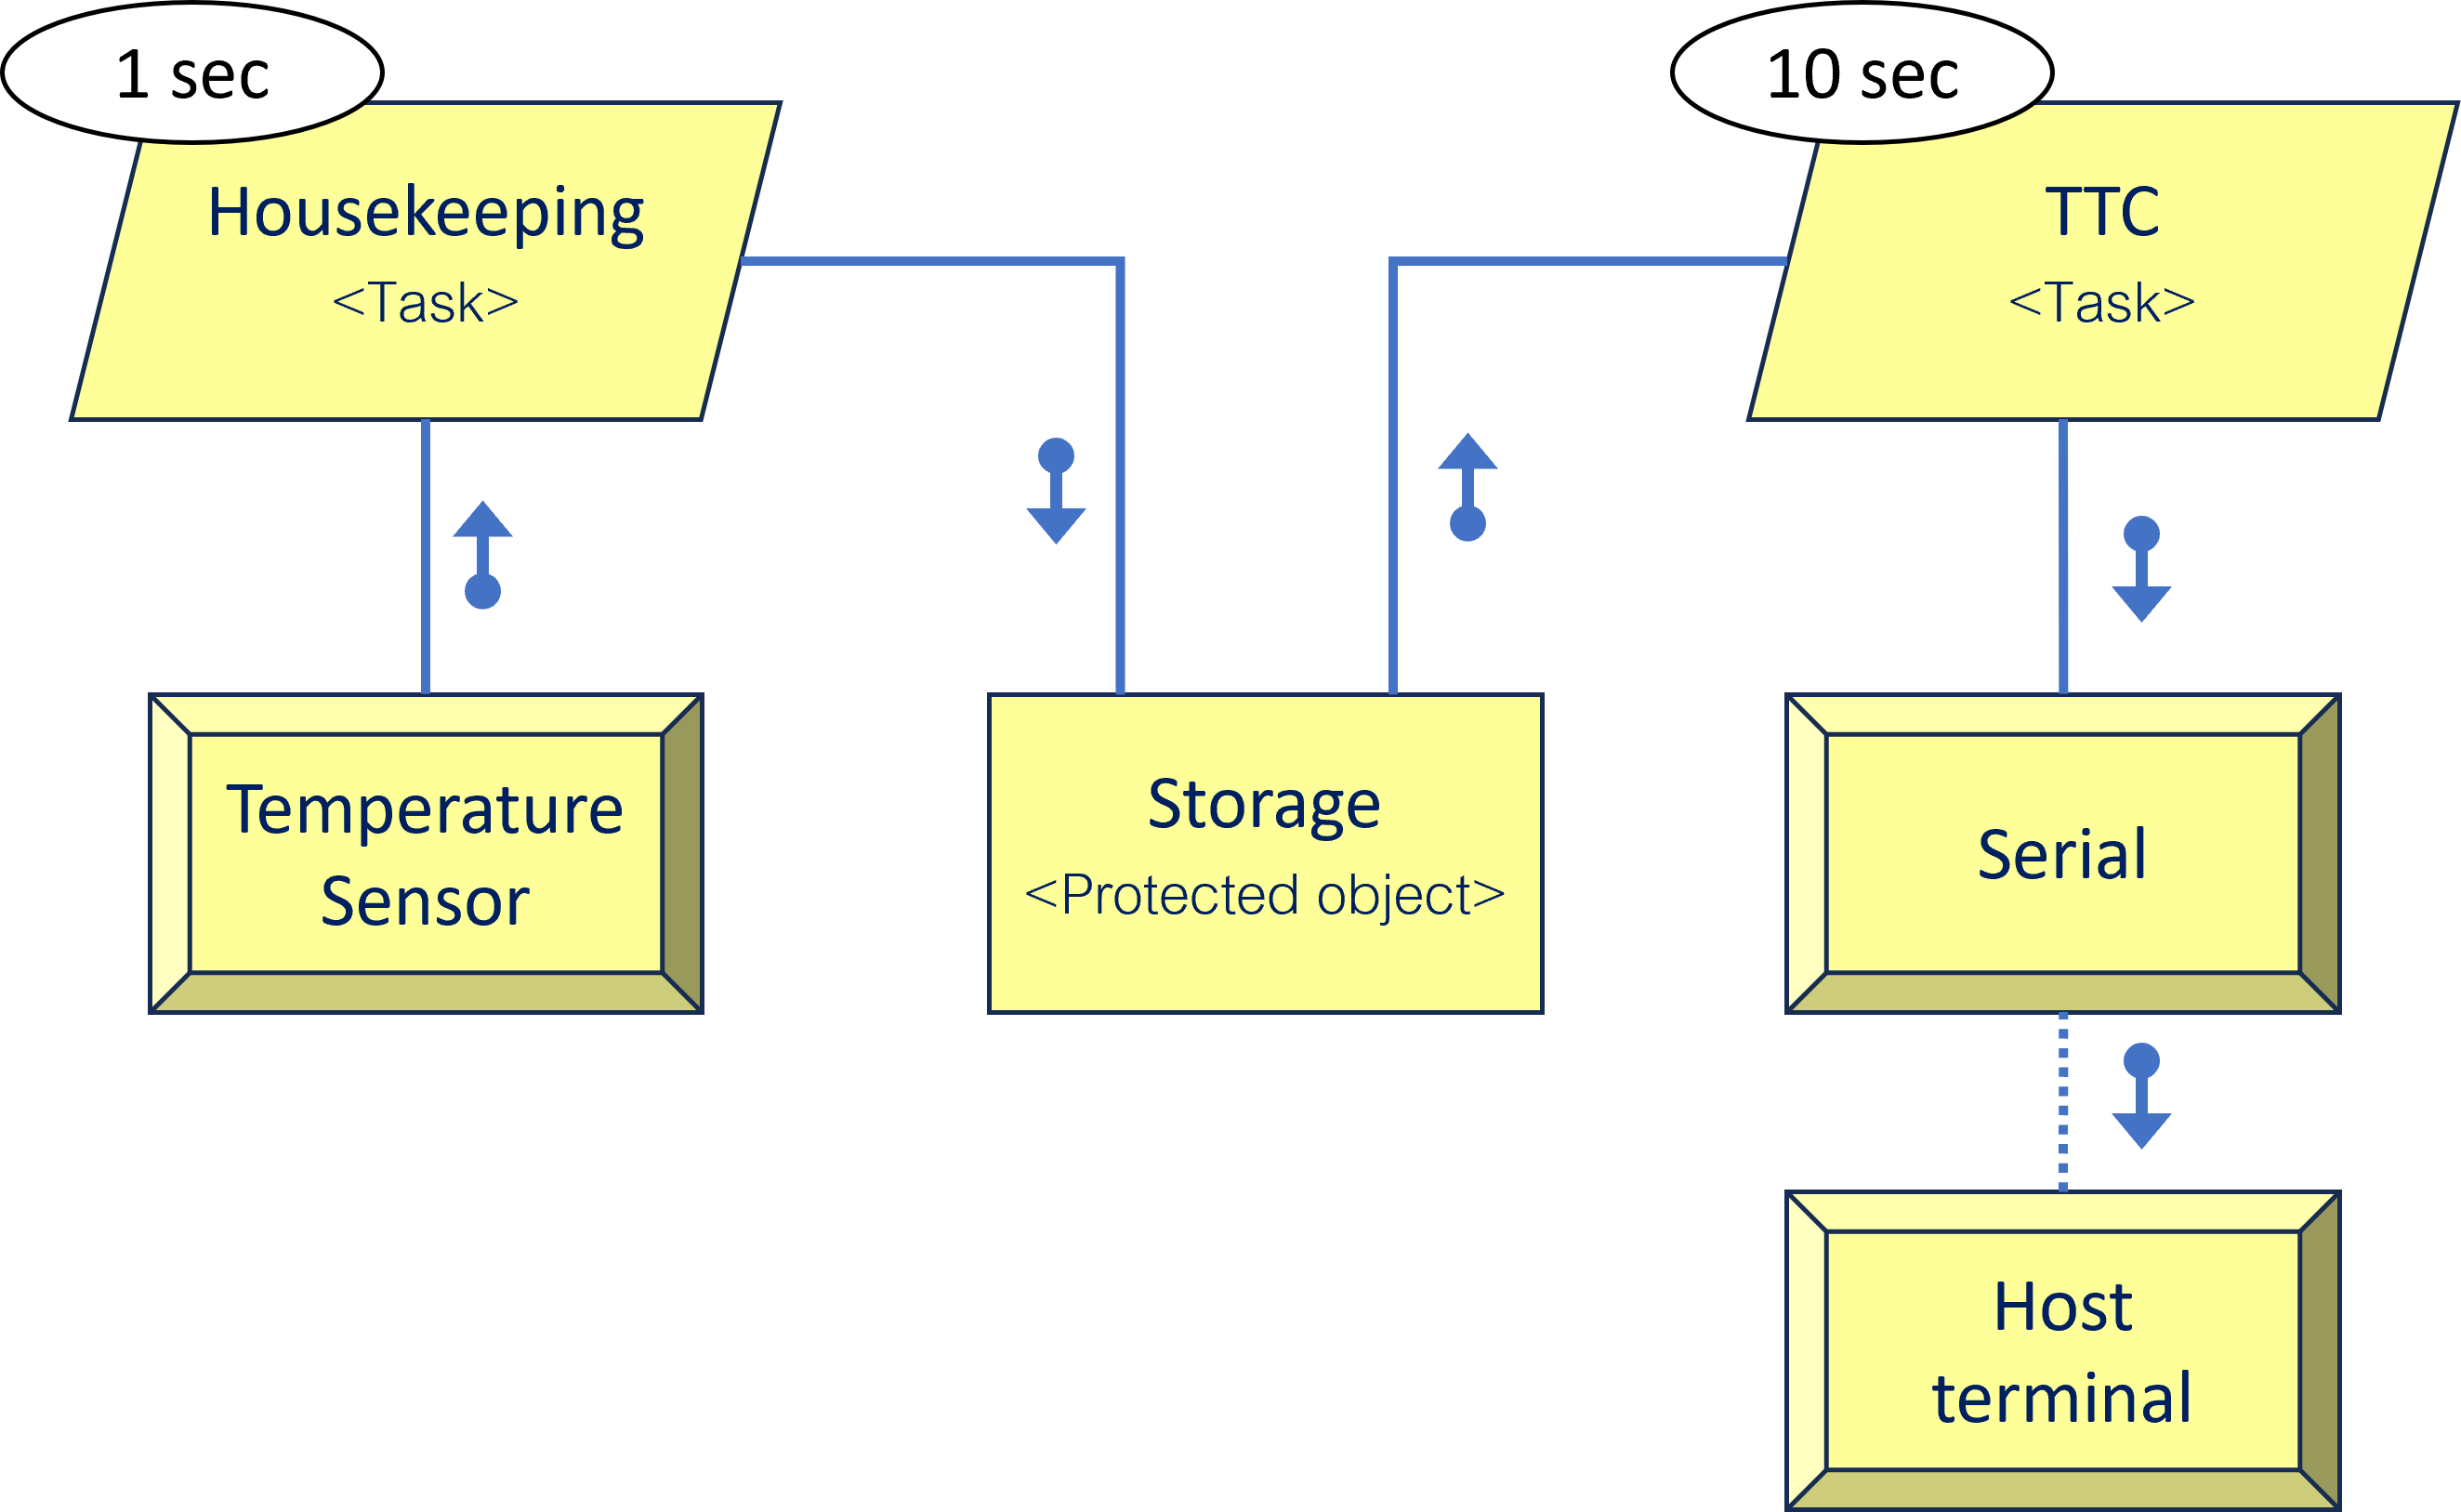
\includegraphics[width=0.8\textwidth,keepaspectratio]{obsw-v2.png}}
	\caption{Software architecture of the OBSW.}
	\label{fig:obdh}
\end{figure}

\begin{description}
\item[Telemetry and Telecommand (TTC).] This component is in charge of the communications with the ground station. The ground station is simulated by the Host terminal. the \texttt{TTC} must be activated cyclically with a 10 second period.

\item[Serial.] This component provides a high-level interface to a text console
where the measured temperature values can be transmitted.

\item[Housekeeping.] Main component,
which performs the basic functionality of the system.
It reads a temperature value and stores it in the \texttt{Storage} component.
It must be activated cyclically with a 1 second period.

\item[Sensor.] This component provides a high-level interface to the temperature sensor and deals with all the details of reading the ADC to which the sensor is connected.

\item[Storage.] This component is a data object storing one temperature value, which is written by \texttt{Housekeeping} and read by \texttt{TTC}. As it is accessed concurrently by two tasks, it must be a protected object guarantying the mutual exclusion.

\end{description}

Since the OBC board does not have a text output device,
temperature values are sent by a serial line to the ground station.
In this way, the radio link between
the satellite and the ground station is
simulated by the \texttt{Serial} and \texttt{Host Terminal} connection (dashed line).

\section{Serial line connections}

This scheme makes use of the USB/UART interface cable provided to the students. The USB/ UART cable has a TTL connector that must be connected to the STM32f4 board pins that convey the serial line (UART) signals (figure~\ref{fig:cable}).

\begin{figure}[h]
    \centering{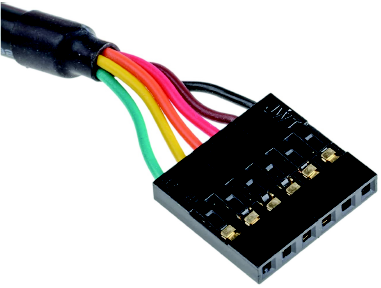
\includegraphics[width=0.3\textwidth,keepaspectratio]{connector.png}}
    \caption{UART cable connector.}
    \label{fig:cable}
\end{figure}

The connections to be made are summarized in the following table (see figure~\ref{fig:board} for the location of the pins on the board):

\begin{table}[htb]
\begin{center}
\begin{tabular}{ll} \hline
Connector pin & Board pin \\ \hline
1 (black) & GND \\
4 (orange) & PB7 \\
5 (yellow) & PB6 \\ \hline
\end{tabular}
\caption{Serial line connections on board.}
\label{tb:connections}
\end{center}
\end{table}

The other end of the interface cable has a USB-A connector
that must be plugged to a USB port on the host computer.
The values sent to the host computer are displayed using a terminal application
that can handle a USB serial port.
The host terminal application should be set to taking the USB serial port as input with
a transmission rate of 115200 bps and
a configuration of 8N1 (8 data bits, no bit parity, 1 bit for stop).

\section{Host terminal application}\label{sc:term}
\subsection{Windows}

The recommended application to display messages received on the USB serial port is PuTTY. You can download an installation package from \url{https://www.putty.org}.

In order to configure the application, you need first to identify the COM port corresponding to the USB serial line. Open the Device Manager and look at the USB Serial Port entry. The COM port is displayed next to it (e.g. COM4 in figure~\ref{fig:com}).

\begin{figure}[hbtp!]
            \centering{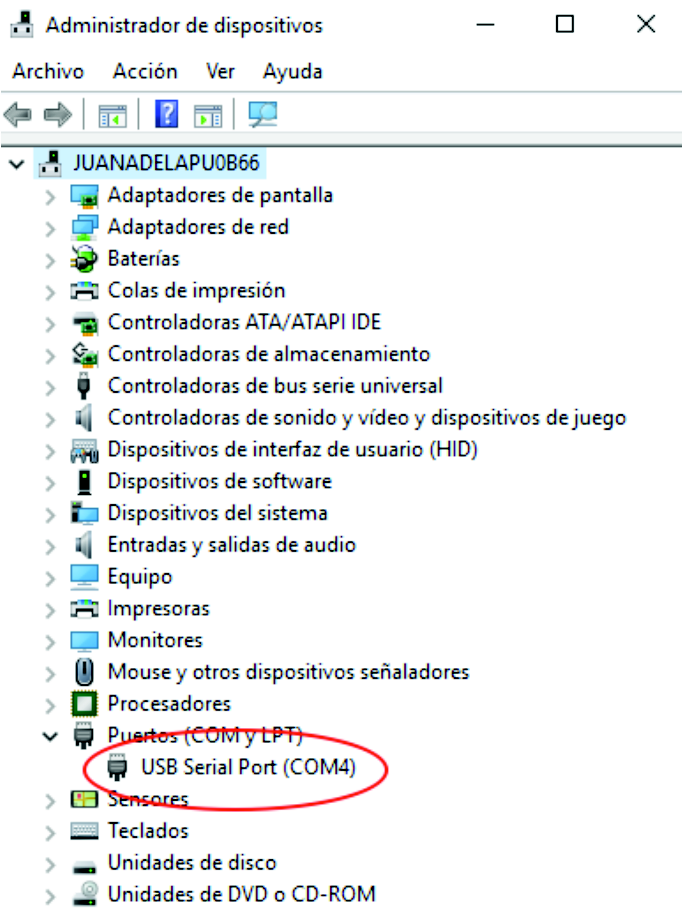
\includegraphics[width=0.6\textwidth,keepaspectratio]{com.png}}
            \caption{Identification of usb serial port.}
            \label{fig:com}
\end{figure}

Now, to set up PuTTY, open the application and set the configuration parameters as shown in figure~\ref{fig:cable}.

\begin{figure}[hbtp!]
            \centering{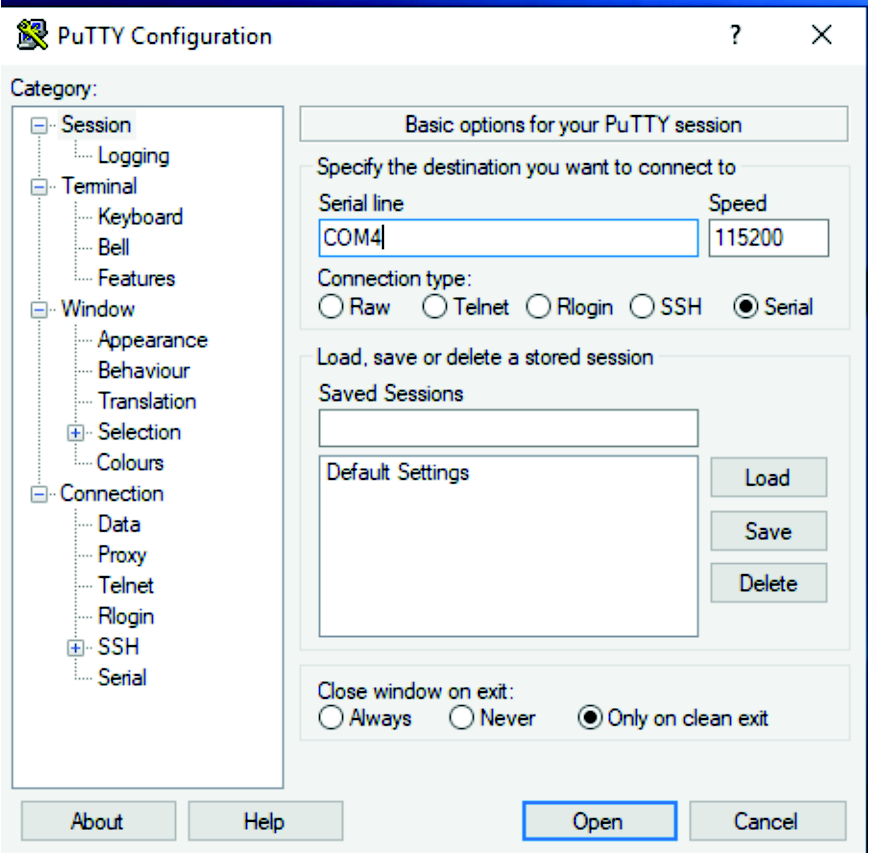
\includegraphics[width=0.6\textwidth,keepaspectratio]{putty.png}}
            \caption{PuTTY configuration.}
            \label{fig:putty}
\end{figure}

\subsection{MacOS}
The recommended application is screen, which is already installed in MacOS.
First you have to identify the USB serial port. Open a terminal window and type

\begin{BVerbatim}
	$ ls /dev | grep -i usb
\end{BVerbatim}

You will get a list of devices like the following:

\begin{BVerbatim}
	cu.usbserial-FTA5I24G
	tty.usbserial-FTA5I24G
\end{BVerbatim}

As you can see, there are two devices for each serial line. You can use any of them, but for reasons not to be discussed here it is better, in general, to use the one starting with cu.

To use the screen application enter the following command:

\begin{BVerbatim}
	$ screen /dev/cu.usbserial-XXXX 115200
\end{BVerbatim}
	
where \texttt{/dev/cu.usbserial-XXXX} is the name of your device.

To exit the application, type CTRL-A and then CTRL-K.

\subsection{GNU Linux}

The recommended application is screen,4 which can be installed in Ubuntu Linux with:

\begin{BVerbatim}
	$ sudo apt install screen
\end{BVerbatim}

In order to identify the USB serial port, type the following command on a terminal:

\begin{BVerbatim}
	$ ls /dev | grep -i usb
\end{BVerbatim}

You will get a result like the following:

\begin{BVerbatim}
	ttyUSB0
\end{BVerbatim}

To use the screen application enter the following command:

\begin{BVerbatim}
	$ screen /dev/ttyUSB0 115200
\end{BVerbatim}

To exit the application, type CTRL-A and then SHIFT-K.

\section{Download the code and study the implementation}

The implementation code, as initially provided to the students, can be downloaded from

\begin{center}
	\begin{tcolorbox}[width=0.6\textwidth,
		boxsep=0pt,
		left=0pt,
		right=0pt,
		top=5pt,
		]
		\centering
		\color{blue}{\url{https://github.com/STR-UPM/SEU-OBDH-Lab}}
	\end{tcolorbox}
\end{center}
 
You can clone the repository or download it as a zip archive.
The code for this assignment is located in the \textcolor{mPurple}{\texttt{lab-3}} folder.

The software components presented in the software architecture section
(figure~\ref{fig:obdh})
are implemented in Ada as packages.
Specifically, the \texttt{Housekeeping} package is the root element of the housekeeping
component.
Its specification consists of one procedure called \texttt{Initialize}
that starts the operation of the component.
The \texttt{Housekeeping} has four subpackages:

\begin{description}
\item[Housekeeping] is the root package of the subsystem and contains a concurrent task, Housekeeping\_Task that stores Data in Storage and toggles the blue LED every second.

\item[Housekeeping.Data] contains the definitions of the data types used in the subsystem. The data type \texttt{Analog\_Data} is used to read the ADC, which are integers in the range 0 to 4095 ($2^{12}-1$) as directly provided by the 12-bit ADC.
The data type \texttt{State} is a record that contains the ADC reading and the corresponding timestamp.

These ADC values have to be converted to engineering units. i.e. degrees Celsius, by following the specification of the temperature sensor (se appendix~\ref{ap:sensor}).
Unless the sensors readings must be used to contorl the satellite,
raw readings are usually sent to ground station
that is in charge of converting them to engineering units.
This way, the OBSW is kept as simple as possible.

\item[Housekeeping.Sensor]  is a low level component
that contains the implementation details of the temperature sensor.
Its specification includes the \texttt{Initialize} and \texttt{Get} procedures.
This package uses the Ada Drivers Library to interact with the OBC board hardware.

\item[Housekeeping.Images] includes functions which are used to convert the temperature and timestamp values to Strings. These functions are called \texttt{Image} per the Ada language conventions,
similar to \texttt{printf} in $\ast$nix environments.
\end{description}

The \textbf{TTC} package is the root of the telecommunications system, which in this version is greatly simplified with respect to a real application.
It contains a concurrent task,
\texttt{HK\_Task},
which periodically obtains the sensor measurements located in the \texttt{Storage} and sends them to the ground station by using \texttt{Serial}.
This activity is performed with a period of ten seconds.
The task also toggles the orange LED for a visual inspection.

The \textbf{Storage} package implements the communication between the \texttt{Housekeeping} and \texttt{TTC} subsystems. 
Since this object is shared by two concurrent tasks, it is implemented as a \textit{protected object},
so that its operations are executed in mutual exclusion.
There is also \textit{conditional synchronization}:
the \texttt{TTC} task must wait until there is a fresh value in the store.
However, \texttt{Housekeeping} should not wait if the previous values put into Storage have not been consumed, in order not to delay the housekeeping function.
In this case, the stored value is overwritten. Notice that this differs from the classical specification of a bounded buffer.

The \textbf{Serial} component is implemented by the \texttt{Serial.IO} package and other packages in the \textcolor{mPurple}{\texttt{serial\_ports}} folder.
These packages have been adapted from the examples in the Ada Drivers Library.
The blocking kind of serial port was chosen for this project.
This means that the task calling the \texttt{Put} operation (\texttt{TM\_Task}) waits on a busy loop (aka. active wait) until the operation is complete.

The main procedure is \textbf{OBSW}.
It calls \texttt{Housekeeping.Initialize},
which initializes the sensor so that \texttt{Housekeeping\_Task} can proceed.
Additionally, the green LED is toggled on and off to provide a visual check that the program is running.

Notice that \texttt{Run}, and hence \texttt{Initialize} and \texttt{OBSW}, never return. Therefore the program executes indefinitely, as is common in embedded systems.
Also note that the Main task runs at the lowest priority level
(\textcolor{mGreen}{\texttt{Main.ads:23:}} \textcolor{blue}{\texttt{with Priority => System.Priority'First}}) to let other components run when they are active.

\section{Compile and run}\label{sec:ass-2:compile-run}

Open GPS and do the following:
\begin{enumerate}
\item Select Open project on the welcome window. Navigate to the \textcolor{mPurple}{\texttt{SEU-OBDH-Lab/lab-3}} directory and open the \texttt{realtime\_housekeeping.gpr} project file.
\item Build the executable and load it into the board by clicking on the \hbox{
\includegraphics[width=1.5em]{buildandload.png}} symbol in the tool bar (or select Build $\rightarrow$ Bareboard $\rightarrow$ Flash to board on the top menu).

The program will be compiled, and the executable will be loaded into the board flash memory. After that, the program starts to run on the board (check the blinking LEDs).
\item Connect the serial cable to a USB port on the host computer, if not already done.
\item Identify the serial port name on the host computer and launch the remote terminal application as explained in section~\ref{sc:term}. The sensor measured values together with their respective timestamps will start being displayed on the host application (figure~\ref{fig:output}).
\end{enumerate}

\begin{figure}[h]
            \centering{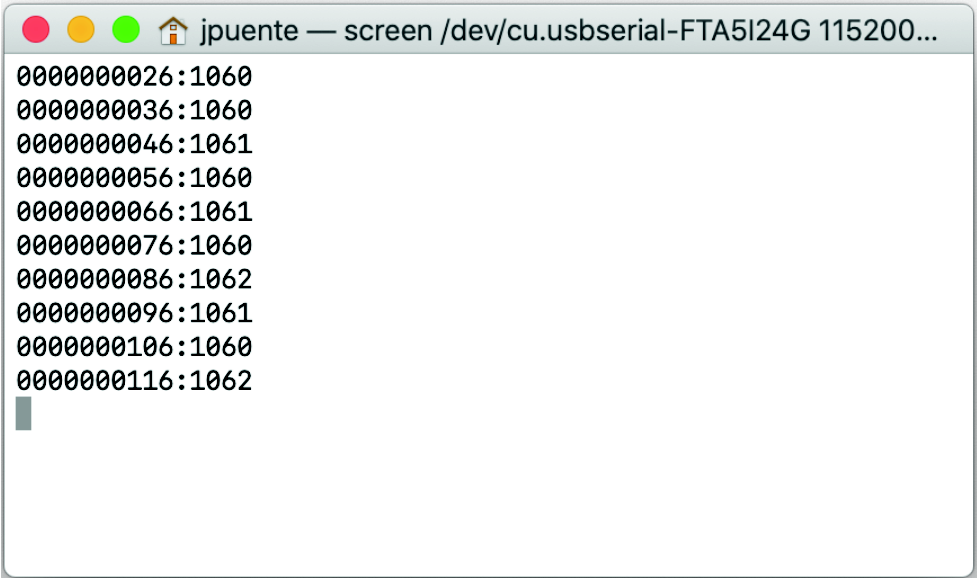
\includegraphics[width=0.6\textwidth,keepaspectratio]{output.png}}
            \caption{Sample output on host terminal.}
            \label{fig:output}
\end{figure}

\section{Make changes to the program}

It is advised that you may make changes
to the provided program in order to make sure
that you understand the project implementation,
and the mapping from the architecture to source code.

\textcolor{mRedBrown}{\textit{The proposed change is to}}: Include the conversion to Celsius in the \texttt{TTC.Send} procedure.
The temperature transfer function is implemented by \texttt{HK\_data-converter}
which can be found in utilities.

\section{Perform a temporal analysis of the system}\label{sc:ta}

Real-time systems need to fulfill temporal requirements,
like activation patterns (cyclic/periodic or sporadic),
the activation periods of the tasks,
or guaranteeing the \textit{schedulability} of the system.
The latter ensures the \textit{temporal behaviour} of the system,
which means that \textit{all tasks
execute within their deadlines}.
This is assured analytically by conducting a \textbf{Response-Time Analysis (RTA)}.
To perform the RTA, you will need to measure the execution time of the task bodies and the protected procedure bodies.
A simple loop technique using the standard real-time clock will be enough for this assignment.

An execution time measurement tool is available in the \textcolor{mPurple}{\texttt{lab-3}} directory.
In order to use it, perform the following steps:

\begin{enumerate}
\item Open GPS and select Open project on the welcome window. Navigate to the \textcolor{mPurple}{\texttt{lab-3}}
directory and open the \texttt{wcet\_meter.gpr} project file.

\item Build the executable and load into the board in the same way as for the \texttt{realtime\_housekeeping.gpr} project, see section~\ref{sec:ass-2:compile-run}.

\item Make sure that the serial cable is still connected to the board and the USB port in the host
computer. If the remote terminal application is not open, open it.
\end{enumerate}

A measurement test is executed on the board, and repeated every 60 s. The output of the test is shown on the host terminal application (figure~\ref{fig:wcet}). The output shows the execution times for the bodies of the Housekeeping (HK) and TTC (TC) tasks, as well as the bodies of the protected operations of the Storage object (ST). Notice that a new entry, \texttt{Get\_Immediate},
has been added for the latter in order \textit{to avoid the measuring task to get blocked}.
The new entry is exactly the same as \texttt{Get} but has a True barrier so that it is always open.

\begin{figure}[h]
    \centering{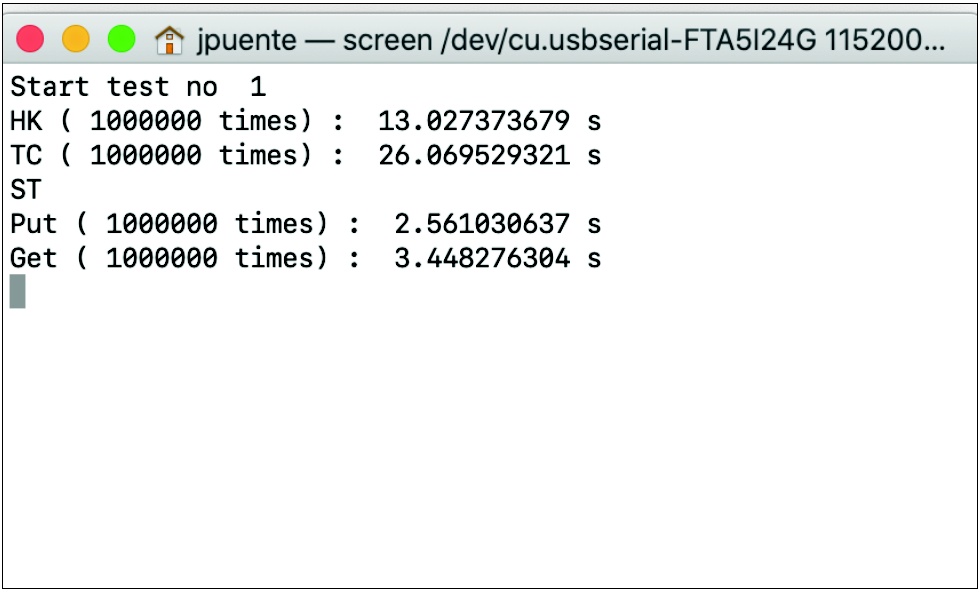
\includegraphics[width=0.6\textwidth,keepaspectratio]{wcet.png}}
    \caption{Output of wcet measurement tool.}
    \label{fig:wcet}
\end{figure}

In the example shown on figure~\ref{fig:wcet}, the HK execution time has been measured $10^{6}$ times, with a total measurement time of 13.02 s. Therefore, the value to be taken for the response time analysis is $13.02\cdot10^{-6}~s = 13.02~\mu${s}, and the same for the other tasks. Take into account that the values measured on your board will probably be slightly different from the above shown.

Once you have an estimate of worst case execution times, apply the RTA equations for computing the worst-case response time and check if all the deadlines are met. The setup for the calculations is shown on table~\ref{tb:wcet}
containing the period (T), execution time (C),
blocking time (B), deadline (D),
response time (R), priority (P),
and accesses to protected object of each task.

\textcolor{mRedBrown}{\textbf{Important}}: The temporal analysis (RTA) will be explained later in the course. Therefore, execution times should be stored for later. 

\begingroup
\setlength{\tabcolsep}{8pt} % Default value: 6pt
\renewcommand{\arraystretch}{1.2} % Default value: 1

\begin{table}[htb]
\begin{center}
	
	\small % Font size
	
	\begin{tabular}{|r r r r r r r r r|} \hline
	\textbf{Task} & T & C & B & D & R & P & Storage & Operation\\ \hline
	
	\textbf{Housekeeping} & 1.0 & $13\cdot10^{-6}$ & \textcolor{mRedBrown}{\textbf{?}} & 1.0 & \textcolor{mRedBrown}{\textbf{?}} & 20 & $3\cdot10^{-6}$ & CPut \\
	
	\textbf{TTC} & 10.0 & $26\cdot10^{-6}$ & \textcolor{mRedBrown}{\textbf{?}} & 2.0 & \textcolor{mRedBrown}{\textbf{?}} & 10 & $4\cdot10^{-6}$ & CGet \\ \hline
	
	& & & & & & CP & \multicolumn{2}{|c|}{\textcolor{mRedBrown}{\textbf{?}}} \\ \hline
	\end{tabular}
	\caption{Data arrangement for RTA of the housekeeping system. Time units in seconds.}
	\label{tb:wcet}
\end{center}
\end{table}

\endgroup

